\documentclass[12pt]{article}
\usepackage[utf8]{inputenc}
\usepackage{amsmath}
\usepackage{comment}
\usepackage{url}
\usepackage{mathtools} % \coloneqq and \eqqcolon
\usepackage{color} 
\usepackage{pgfplots,tikz}

% BIBLIOGRAPHY
\usepackage[sort]{natbib}
%\bibliographystyle{abbrvnat}
\bibliographystyle{plainnat}
\setcitestyle{authoryear}

\setlength{\textwidth}{6.5in}
\setlength{\oddsidemargin}{0.00in}      
\setlength{\topmargin}{-0.4in}
\setlength{\headheight}{0in}
\setlength{\textheight}{9.0in}  

\setlength{\parindent}{0em}
\setlength{\parskip}{1em}
%\renewcommand{\baselinestretch}{1.0}

\def\Eq#1{Eq.~\ref{#1}}
\def\Eqs#1#2{Eqs.~\ref{#1}--\ref{#2}}
\def\EqsAnd#1#2{Eqs.~\ref{#1} and \ref{#2}}

\def\Sec#1{Sec.~\ref{#1}}
\def\Secs#1#2{Secs.~\ref{#1}--\ref{#2}}
\def\SecsAnd#1#2{Secs.~\ref{#1} and \ref{#2}}

\def\Fig#1{Fig.~\ref{#1}}
\def\Figs#1#2{Figs.~\ref{#1}--\ref{#2}}
\def\FigsAnd#1#2{Figs.~\ref{#1} and \ref{#2}}

\def\myline{\centerline{\rule{13cm}{0.4pt}}}

\def\MGluTwoFiveHTTwoA{\MGluTwo/\FiveHTTwoA}
\def\MGluTwo{mGlu$_2$}
\def\MGluTwoThree{mGlu$_{2/3}$}
\def\FiveHTTwoA{5-HT$_{\rm 2A}$}
 
\def\ca{{\rm Ca}^{\rm 2+}}
\def\Ca{$\ca$}
\def\Ip{${\rm IP}_3$}
\def\Ipr{${\rm IP}_3{\rm R}$}
\def\CaiConc{[\Ca]$_i$}
\def\LY{LY379268}

\def\G{{\rm G}}
\def\H{{\rm H}}
\def\GG{{\rm GG}}
\def\GH{{\rm GH}}
\def\HH{{\rm HH}}
\def\GGH{{\rm GGH}}
\def\GHH{{\rm GHH}}
\def\GGHH{{\rm GGHH}}

\def\g{[\G]}
\def\h{[\H]}
\def\gg{[\GG]}
\def\gh{[\GH]}
\def\hh{[\HH]}
\def\ggh{[\GGH]}
\def\ghh{[\GHH]}
\def\gghh{[\GGHH]}

\def\gtot{G_T}
\def\htot{H_T}

\title{Research Notes: Expression ratio-dependent \MGluTwoFiveHTTwoA\ 
cross-talk}
\author{Greg Conradi Smith (w/ Javier and Spenser)}
\date{\today}

\begin{document}

\maketitle
\thispagestyle{empty}

\section*{\boldmath Reproducing the observation of Moreno et al. 2016}
 
  \MGluTwoThree\ receptor agonist \LY\ induced increases in \CaiConc\ in HEK 293 cells that coexpress the \MGluTwo\ and \FiveHTTwoA\ receptors \citep{MorenoEtal16}.  The amount of functional cross-talk (response) depends upon the ratio of expression levels of these receptors (\MGluTwo:\FiveHTTwoA\ of 1:1, 1:2, and 1:3).  Javier mentioned that it seems counter-intuitive for the response would be a  bi-phasic function of the relative expression level.  
 
  
\begin{figure}[h!]
    \centering
    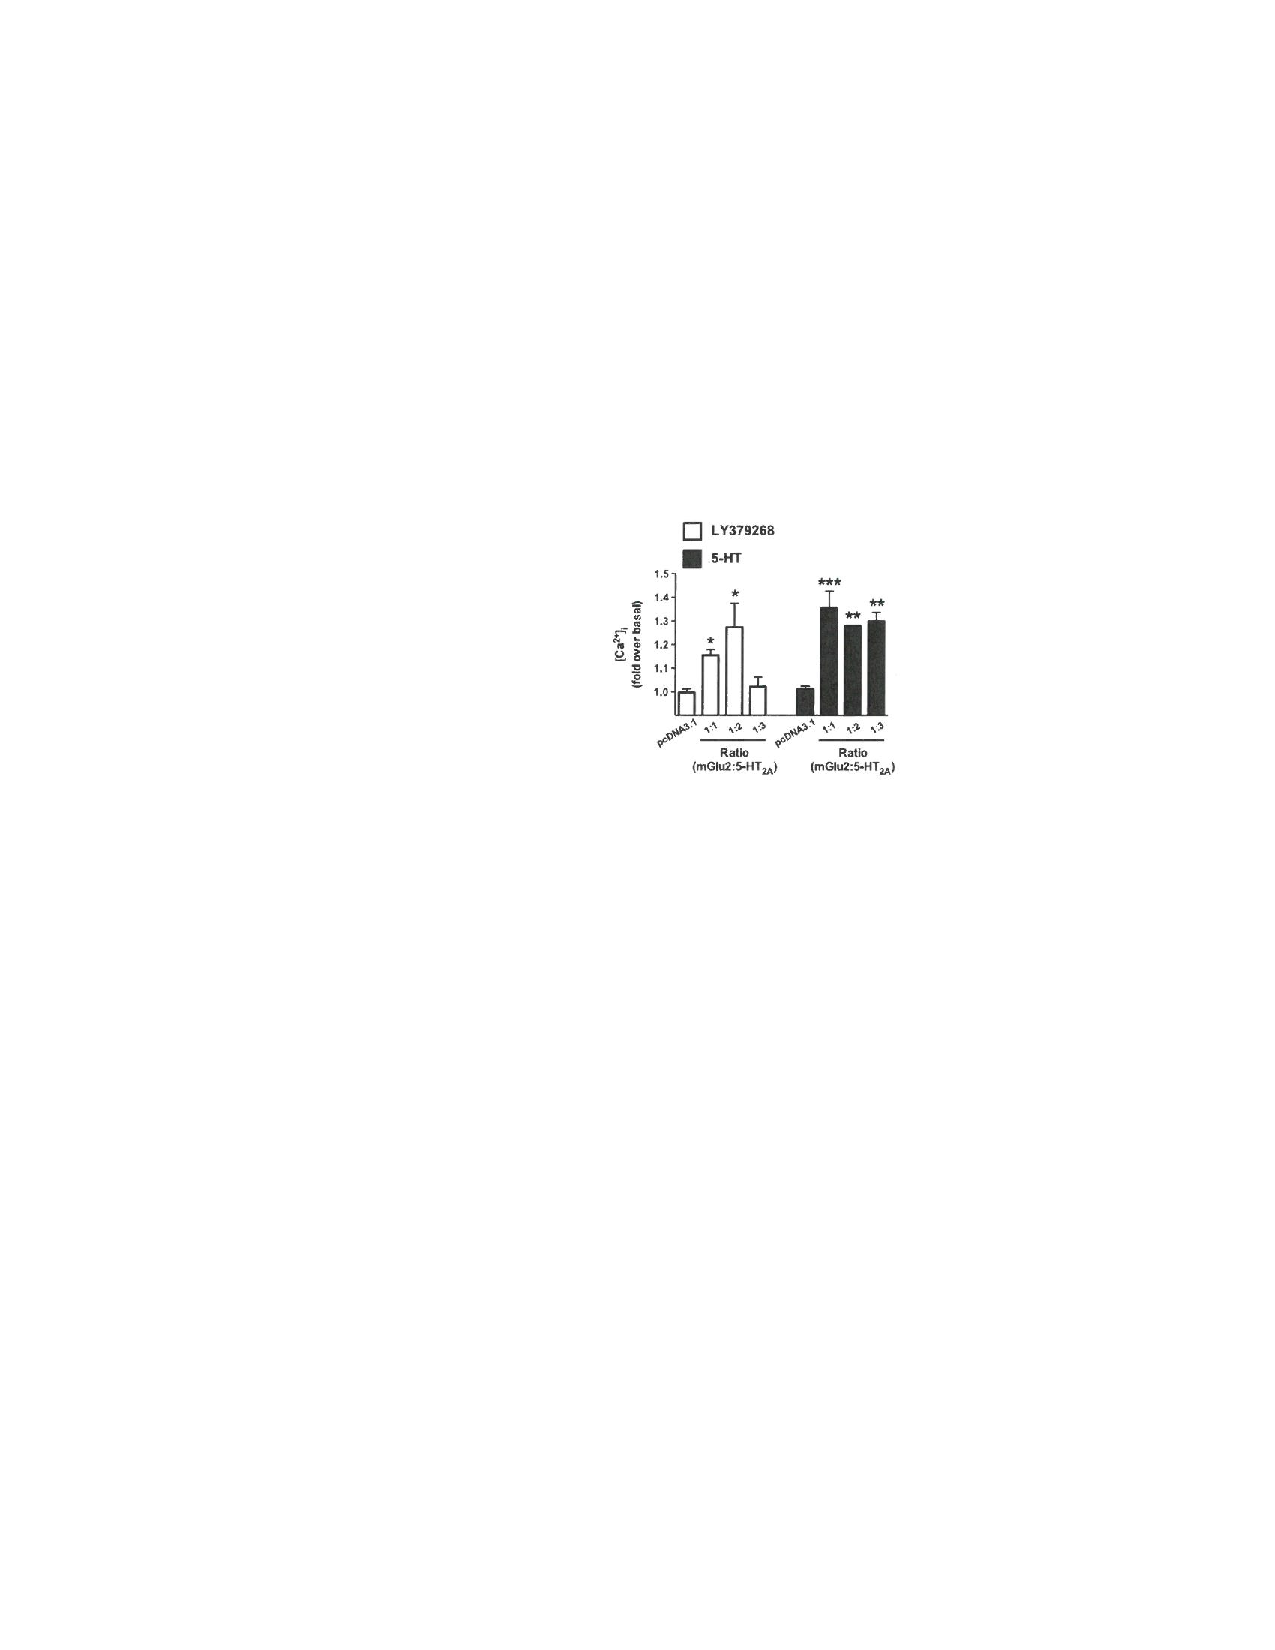
\includegraphics[width=0.4\textwidth]{FigMorenoEtal2016Fig1d.pdf}
    \caption{Panel D from \cite{MorenoEtal16}. }
    \label{MorenoEtal}
\end{figure}

\subsection*{\boldmath Possible explanation}

Greg's intuition suggested the following possible explanation.  If the (cross-talk) response were (for some reason) dominated by \GGH\ heteromers (as opposed to \GGHH), then perhaps this would explain the observed dependence of response on relative expression levels.   The model presented below shows that is is the case.

\subsection*{\boldmath Model of dimerization and heterodimerization}

Let \G\ be the \MGluTwo\ monomer, \H\ be the \FiveHTTwoA\ monomer, \GG\ and \HH\ the homodimers, etc. The species would be \G, \GG, \H, \HH, \GGH, \GHH, \GGHH\ (always writing \G's before \H's, order of symbols does not matter).

The total amount of \G\ and \H\ are given by, respectively, 
\begin{eqnarray}
\gtot & =& \g + 2 \gg + \gh + \ghh + 2\ggh + 2\gghh \label{GTOT}\\
\htot &=& \h + 2 \hh + \gh + 2 \ghh  + \ggh  + 2\gghh  \label{HTOT} \, . 
\end{eqnarray}

\begin{figure}
    \centering
 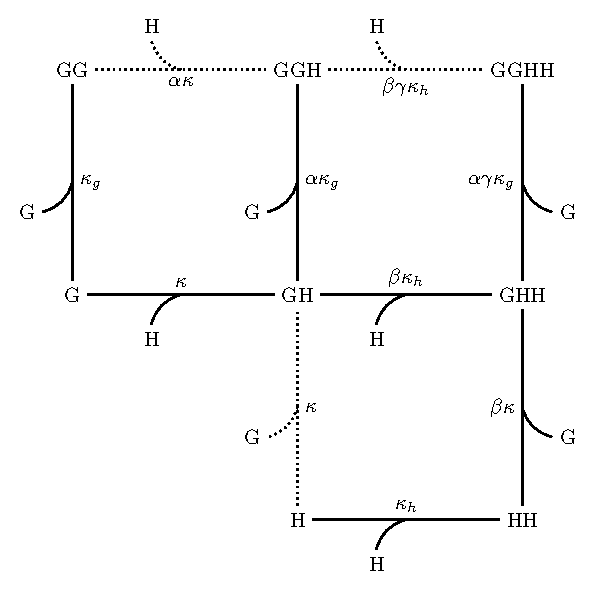
\includegraphics[width=0.6\textwidth]{FigGHDiagram.pdf}  
    \caption{Diagram of bimolecular association reactions, equilibrium association costants, and allosteric parameters. Reactions used to derive \Eqs{EquilibriumRelationsA}{EquilibriumRelationsB} are shown solid.}
    \label{fig:diagram}
\end{figure}

The equilibrium relations are:
\begin{eqnarray}
\hh & = & \kappa_h \h^2 \label{EquilibriumRelationsA}\\
\gg & = & \kappa_g \g^2 \\
\gh & = & \kappa \g \h  \\
\ggh & = & \alpha \kappa_g \g \gh = \alpha \kappa \gg \h  \label{EquilibriumRelationsGGH}   \\
\ghh & = & \beta \kappa_h \gh \h  = \beta \kappa \g \hh  \\
\gghh & = & \alpha \gamma \kappa_g \g \ghh  = \beta \gamma \kappa_h  \ggh \h   \label{EquilibriumRelationsB}
\end{eqnarray}
This allows us to write \Eqs{GTOT}{HTOT} as polynomial functions of $\g$ and $\h$:
\begin{eqnarray}
\gtot & = & \g + 2 \kappa_g \g^2 + \kappa \g \h \\
&+& 2 \alpha \kappa_g \kappa \g^2 \h  + \beta \kappa_h \kappa \g \h^2  + 2 \alpha \beta \gamma \kappa_g \kappa_h \kappa \g^2\h^2 \label{GTOTAgain}\\
\htot &=& \h + 2 \kappa_h \h^2  +  \kappa \g \h \\
&+&  \alpha \kappa_g \kappa \g^2 \h + 2 
\beta \kappa_h \kappa \g \h^2     + 2 \alpha \beta \gamma \kappa_g \kappa_h \kappa \g^2\h^2 \label{HTOTAgain}
\end{eqnarray}

Define $f_G(\g,\h) := \gtot - ( \g + 2\kappa \g^2 + \cdots + 2 \alpha \beta \gamma \kappa_g \kappa_h \kappa \g^2\h^2 ) $
and similarly for $f_H(\g,\h)$, and notice that $f_G$ and $f_H$ are both increasing functions of $\g$ and $\h$.  For this reason is straightforward to numerically calculate the equilibrium concentrations of \G\ and \H.  The answer depends on the chosen parameters:   two expression levels, i.e., the total concentrations $\gtot$ and $\htot$,  three equilibrium association constants ($\kappa_g$, $\kappa_h$, $\kappa$), and three allosteric parameters ($\alpha$, $\beta$, $\gamma$).   

\begin{figure}
    \centering
    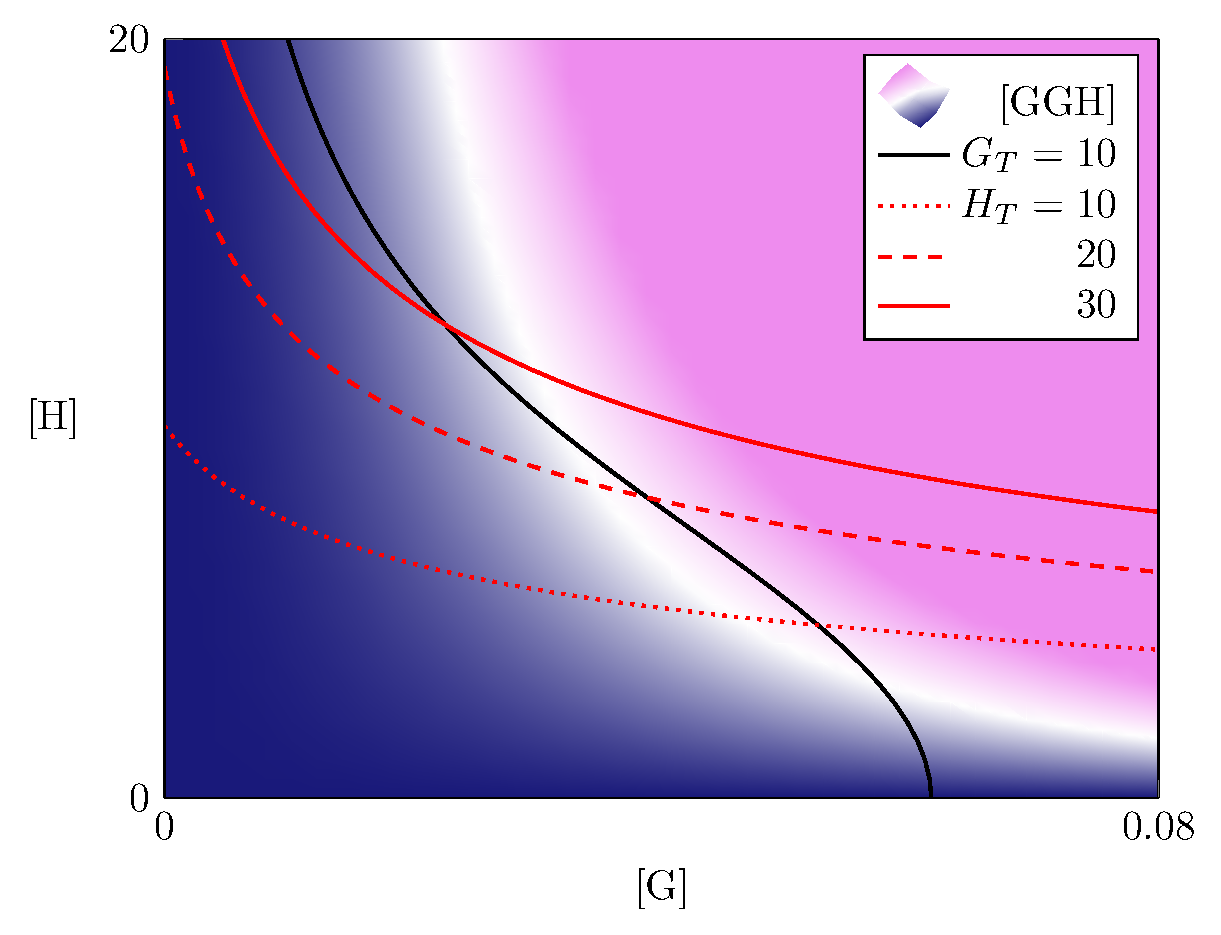
\includegraphics[width=0.7\textwidth]{FigGHRatioStudyLoci.pdf}
    \caption{Contour labels are the total concentrations $\gtot$ (solid) and $\htot$ (dashed). Increased $\htot$  decreases  $\h$ and increases $\g$.  This leads to the decreased response shown in \Fig{FigBars}.}
    \label{FigContours}
\end{figure}

 \Fig{FigContours} shows how these equilibrium concentrations of $\g$ and $\h$ are given by the intersection of the curves $f_G(\g,\h; \gtot)=0$ and   $f_H(\g,\h; \htot)=0$, the locations of which depend on $\gtot$ and $\htot$, respectively.  

In \Fig{FigContours},  three increasing values of $\htot$ are used ($\gtot$ is fixed).  The curve intersections show $\g$ decreasing and $\h$ increasing as the $\gtot:\htot$ expression ratio changes from 1:1 to 1:2 to 1:3.  Assuming that the functional cross-talk is proportional to $\ggh$, this results in a decreasing response (see  \Fig{FigBars}), reproducing the counterintuitive experimental observation of \cite{MorenoEtal16}  shown in \Fig{MorenoEtal}.

%Because of the way the binding processes in \Fig{fig:diagram} are coupled, the equilibrium value of $\GGH$ (and the response) may depends on the ratio of $\htot$ to $\gtot$ (see \Fig{FigBars}).  A parameters search gives the series of three responses shown in \Fig{FigBars}.  

 \begin{figure}
    \centering
     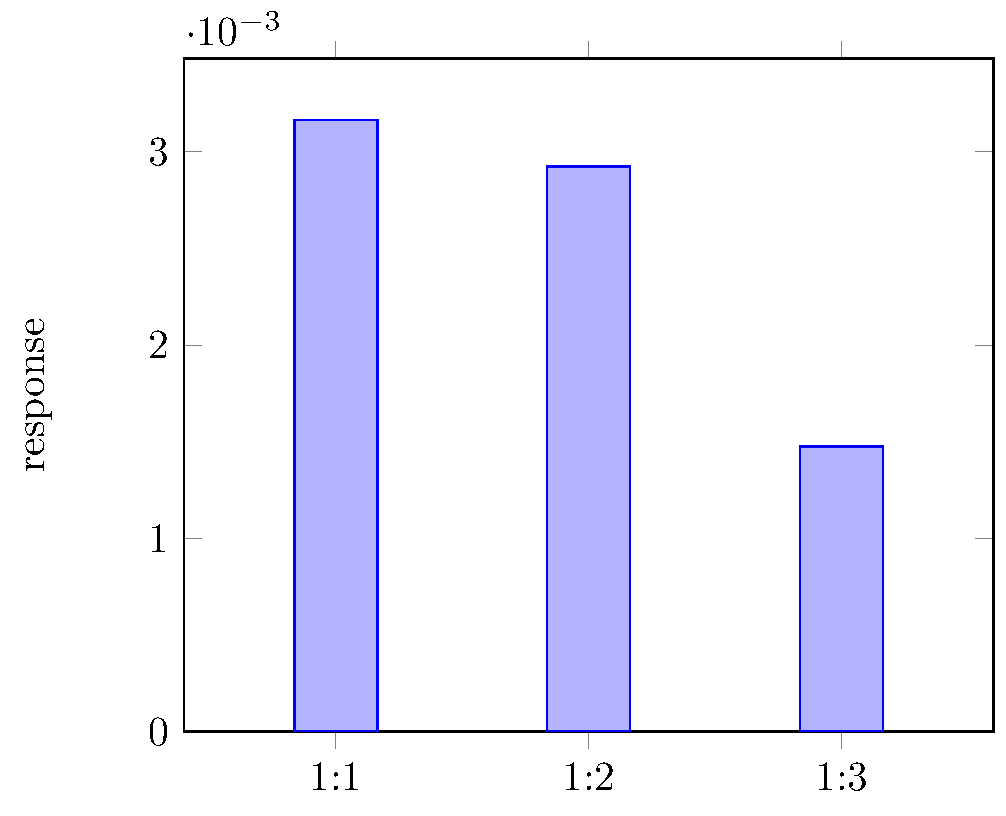
\includegraphics[width=0.4\textwidth]{FigGHRatioStudyBarGraph.pdf}    \caption{Response for three different values of $\gtot:\htot$. Parameters: $\kappa=0.25$, $\kappa_g=1300$, $\kappa_h=0.001$, $\alpha=0.001$, $\beta=10000$, $\gamma=0.001$.  The response is assumed to be proportional to $\ggh$.}
    \label{FigBars}
\end{figure}

\subsection*{For discussion}

\begin{itemize}
\item Many parameter sets do not lead to the counter-intuitive response.  What is it about these parameter values that leads to the counter-intuitive response?  

\item Is there any biological reason to think that the amount of functional cross-talk might be greater in $\GGH$ than $\GGHH$?  (This is the primary assumption that makes the model reproduce the counter-intuitive response, so perhaps we should discuss whether or not this assumption could be biologically realistic.) 

 \end{itemize}

\nocite{MorenoEtal16}
\bibliography{gpcr}

\end{document}





 